\section{Introduction to Blockchain}
\subsection{What is Blockchain}
From a technical point of view, Blockchain is a distributed ledger that is cryptographically
secure, append-only, immutable (extremely hard to change), and updateable only
via consensus among nodes.

From a business point of view, a blockchain can be defined as a platform
whereby peers can exchange values without the need for a central trusted party
by using transactions which are stored inside the blockchain in a verifiable and
permanent way.












\subsection{Blockchain features}

\subsubsection*{Decentralization}
This is the core feature of Blockchain. Thanks to decentralization there's no
need of a central trusted entity which stores the data and validates the
transaction, since the same copy of the Blockchain is stored by every node and
the validation of transaction is achieved through consensus.

\subsubsection*{Distributed consensus}
Blockchain have a high Byzantine Fault Tolerance\footnote{without BFT, a peer
would able to transmit and post false transactions} and allows to achieve
distributed consensus, therefore allows to have a single version of a data value
agreed by all parties without requiring a central authority.

\subsubsection*{High availability}
Blockchain is based on a peer-to-peer network of thousands of nodes and data is
replicated on each node, therefore the whole system is highly available since even
if one or more nodes fail the whole network can continue to work correctly.


\subsubsection*{Immutability}
All the data stored in a blockchain is immutable: once a block has been added to
the blockchain, it is considered pratically impossible to change it (changing it
is computationally infeasible since it would require an unaffordable amount of
computing resources).

\subsubsection*{Transparency}
Blockchain is shared between the nodes and everyone can see what is in the
blockchain, thus allowing the system to be transparent and trusted.

\subsubsection*{Security}
Blockchain ensures the integrity and the availability of the data. Since
private keys and digital signatures are used, it also provide authentication and
non-repudiation. It doesn't provide confidentiality, due to it's transparency
feature (privacy is however required in certain scenarios, thus research in
this area is being carried out).

Blockchain security is due especially to its distributed nature, since for an
attacker would be a lot easier to tamper with data if it was stored on a single
central entity.

\subsubsection*{Uniqueness}
In Blockchain every transaction is unique and has not been spent already.
This is especially usefull in cryptocurrencies applications of Blockchain,
where avoidance of double spending is a key requirement.















\subsection{Blockchain structure}
As shown in figure \ref{fig:blockchain-basic-schema}, a blockchain consists of
linked list of ordered fixed-length blocks, each of which includes a set of transactions.
In this section, the generic elements of a blockchain will be presented.
\begin{figure}[!htb]
	\centering
	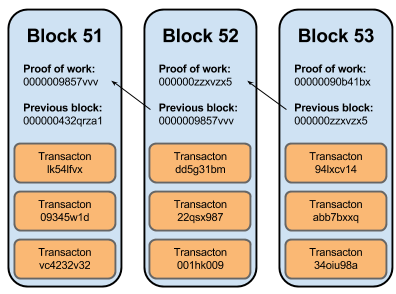
\includegraphics[width=0.5\linewidth]{img/blockchain-basic-schema.png}
	\caption{basic blockchain schema}
	\label{fig:blockchain-basic-schema}
\end{figure}

\subsubsection*{Blocks}
A block groups transactions in order to organize them logically and its size
depends on the blockchain implementation. Generally, a block is composed of:
\begin{itemize}
  \item a set of transactions
  \item a hash which identifies the block
  \item a pointer to the previous block hash (unless it's the genesis block)
  \item a nonce
  \item a timestamp
\end{itemize}
The \emph{genesis block} it's simply the first block in the blockchain and therefore
it can't contain any reference to the previous block.


\subsubsection*{Addresses}
Addresses are unique identifiers which identify the parties involved in a
transaction. An address is usually a public key or it's derived from a public key.


\subsubsection*{Transactions}
A transaction is a tranfer of value from an address to another.


\subsubsection*{Peer-to-peer network}


\subsubsection*{Transaction scripts}
Transaction scripts are predefined sets of commands for nodes to transfer values
from one address to another and perform various other functions.


\subsubsection*{Programming language and Virtual machine}
A Turing-complete programming language is an extension of transaction scripts and
it allows the peers to define the operations that has to be performed on a
transaction, without the limitations of a non-Turing-complete transaction script.
Programs encapsulate the business logic and can for example transfer a value
from one address to another only if some conditions are met.

A virtual machine allows Turing-complete code to be run on a Blockchain as
smart contract (e.g. Ethereum virtual machine).

Not every Blockchain supports Turing-complete programming languages and virtual
machines (e.g. Bitcoin is not Turing-complete\footnote{It however supports
smart contracts}).


\subsubsection*{Nodes}
A node is an active entity which stores a copy of the blockchain and can perform
and/or valide transactions (following a consensus protocol, e.g. the Proof of Work).









\subsection{Consensus in Blockchain}









\subsection{Types of Blockchain}
Blockchain can be distinguished into three different types, each one charaterized
by a certain set of attributes.
\subsubsection*{Public Blockchain}
Public Blockchains are blockchains open to the public in which everyone can join
the network, mantain the shared ledger and partecipate in the consensus process.
The ledger is therefore owned by noone and is publicly accessible by everyone.

These type of Blockchain typically have an incentivizing mechanism to encourage
more participants to join the network. Bitcoin for example, one the largest public
Blockchain, reward with cryptocurrency miners who join the network.

Public Blockchains have two main disadvantages: the substantial amount of
computational power required to maintain a distributed ledger at a large scale
and the lack of privacy for the transactions stored inside the blockchain.  
